\chapter{Photometry of EC2117-54}


\section{Observations}
\label{ch_photometry}

% This chapter describes the methods used to obtain the observational data as well as the methods used to clean, prepare and analyse the datasets.
% 
% For this project measurements of the object's brightness were taken simultaneously with its spectrum. Both the photometric and spectroscopic  measurements were obtained using short exposure times in order to have high time resolution.

\subsection{SAAO 1.9m Radcliff Reflector}

\label{saao1.9}

The photometric observations were made using the 1.9m reflector\footnote{Details of this telescope can be found at http://www.saao.ac.za/facilities/telescopes/19m/} at the South African Astronomical Observatory (SAAO) site in Sutherland. The telescope was built between 1938 and 1948 by Grubb-Parsons. It was originally situated at the Radcliff Observatory outside Pretoria, but was moved to Sutherland in the 1970s due to bad light pollution.

The telescope is equatorially mounted, and is used in a Cassegrain configuration at the f/18 focus. It can be fitted with a variety of instruments, the most common being the University of Cape Town (UCT) CCD photometer, a grating spectrograph and a fibre-fed Echelle spectrograph.



\subsection{UCT CCD Photometer}
\label{uctccd}

The UCT CCD photometer is a Wright Instruments Peltier-cooled camera. It has a 576x420 thinned, back-illuminated EEV CCD. The instrument can be used on the 1.9m, 1.0m and 0.75m telescopes at Sutherland. The instrument is controlled by a 486 computer running MS-DOS \citep{UCTCCD}.

It can be used in various configurations. The gain can be set depending on the brightness of the target objects. The gain is the ratio of photo-electrons to Analog-to-Digital units (ADU). The gain can be set to either 1 or 4 with gain 1 corresponding to 10 photo-electrons/ADU and gain 4 corresponding to 2.5 photo-electrons/ADU. This option is available to optimise signal-to-noise ratios for bright and faint stars. With the gain set to 1, a higher number of photo-electrons can be read before the analog-to-digital converter saturates. This setting is used for bright stars. On a gain setting of 4, a higher number of ADUs are read per photo-electron thereby decreasing the noise added by the readout process.  The gain was set to 4 for all the observations made for this project.

The CCD can be prebinned before the values are read out, in order to reduce readout noise and increase the signal-to-noise ratio. The instrument allows prebinning values from 1x1 to 6x6, however, using too much binning may result in stellar images that are undersampled for precise  Point Spread Function (PSF) fitting. A general rule of thumb is to  select the prebinning such that the star occupies $\sim$2.2 pixels on the output image. The image scale is 0.139 arcsec/pixel on the 1.9m telescope and generally prebinning values of 3x3 or greater are used, depending on seeing conditions.

The CCD is also equipped to perform observations in frame transfer mode. In this mode, half the CCD is masked by a frame transfer mask. The unmasked half is then exposed, after which the counts are transferred to the masked half of the CCD, where they can be read out while the unmasked area is exposed again. This minimises the downtime between exposures. The field-of-view on the 1.9m telescope in this mode is $34''$x$50''$ \citep{woudt2001HSP}. This high-speed mode was used for the observations made for this project.




\subsection{Photometric Observations in 2006}
\label{sub_observations}
Photometric observations of EC2117-54 were made on four consecutive nights from 16 to 19 August 2006. The runs on 18 and 19 August were hampered by intermittent cloud.  The observations were made using a Johnson V filter in order to provide a way of correlating the photometric and spectroscopic observations. An integration time of 6 seconds was selected. This is the highest time resolution that is reliable on this instrument and is well within the Nyquist frequency for the most rapid oscillations that were to be studied. The use of shorter integration times than $\sim6$s causes the computer controlling the camera to crash intermittently, due to the limited speed at which the frames can be transferred across the network.  The shortest timescale of the variations under study is approximately 20 seconds. According to the Nyquist sampling theorem, a signal with frequency $f_{0}$ must be sampled at a frequency of at least $2f_{0}$ to be fully resolved.  The telescope was pointed in such a way that ensured that the image contained at least one relatively bright non-variable star that could be used to calculate differential corrections (Figure \ref{exposure}). Table \ref{obslog} lists the full observation log.


%#############################################################################################################################
\begin{figure}
\centering
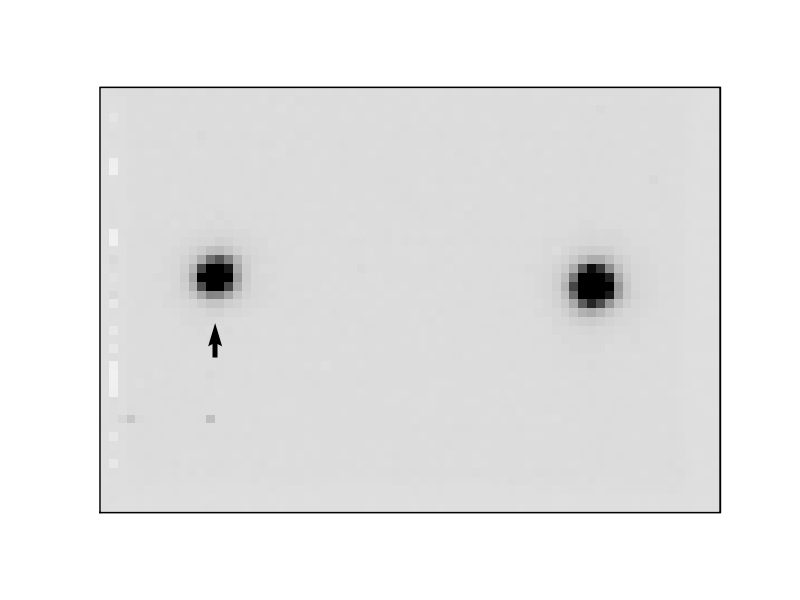
\includegraphics[bb=0 0 600 400,width=0.85\columnwidth]{images/ec2117_phot_exp.png}
% ec2117fits.png: 600x400 pixel, 72dpi, 21.17x14.11 cm, bb=0 0 600 400
\caption[Example of photometric exposure]{Example of photometric exposure of EC2117-54 and comparison star. The arrow marks EC2117-54. The field of view is $34''$x$50''$.}
\label{exposure} 
\end{figure}

\begin{table}
\caption[Photometric Observations Log]{Photometric Observations Log}
\begin{small}
\centering
% use packages: array
\begin{tabular}{lcccccc}
\hline\hline\\ Run No & Date            & HJD of first obs & Length & $t_{in}$ & Tel & Filter \\ 
        &(start of night) &     (+2453900)   &    (h)   & (s) &       & \\\\ \hline  \\
 S7651  & 16 Aug 2006     &    64.28141      &  5.35    & 6  & 74-in & V \\ 
 S7655* & 17 Aug 2006     &    65.32565      &  6.26    & 6  & 74-in & V \\  
 S7659  & 18 Aug 2006     &    66.31921      &  4.36    & 6  & 74-in & V \\ 
 S7661  & 19 Aug 2006     &    67.40985      &  0.74    & 6  & 74-in & V \\\\ \hline \\\\

\end{tabular}
Notes: $t_{in}$ = integration time, V = Johnson V filter, HJD = Heliocentric Julian Date, * = Simultaneous observations with SALT time-resolved spectroscopy.



\end{small}

\label{obslog}
\end{table}

%#############################################################################################################################
%#############################################################################################################################



%#############################################################################################################################



\subsection{Archival Observations}
\label{obs_archive}

In addition to the August 2006 observations, all lightcurves containing eclipses were retrieved from the archive\footnote{All observations of CVs obtained by UCT on SAAO telescopes are stored in an electronic archive.} in order to study the behaviour of rapid oscillations. This is further explained in Sect. \ref{ro_phot_lc}. Table \ref{archive_obslog} displays the archival runs used in the analysis. The observations were all made using the SAAO 40-inch telescope and the UCT CCD photometer. Refer to \cite{WWP} for further details of the observations.



\begin{table}
\caption[Archival Photometric Observations Log]{Archival Photometric Observations Log}
\begin{small}
\centering
% use packages: array
\begin{tabular}{lcccccc}
\hline\hline\\ Run No & Date            & HJD of first obs & Length & $t_{in}$ & Tel & Filter \\ 
        &(start of night) &        &    (h)   & (s) &       & \\\\ \hline  \\

S6544  &   07 Sept 2002   &  2452525.28604  &  6.11  &  6.0 & 40-in & WL \\
S6548  &   01 Oct 2002    &  2452549.30417  &  5.27  &  5.0 & 40-in & WL \\
S6549  &   03 Oct 2002    &  2452551.27063  &  2.34  &  6.0 & 40-in & WL \\
S6551  &   04 Oct 2002    &  2452552.27894  &  3.72  &  5.0 & 40-in & WL \\
S6555  &   06 Oct 2002    &  2452554.23099  &  1.39  &  6.0 & 40-in & WL \\
S6564  &   08 Oct 2002    &  2452556.22808  &  1.95  &  6.0 & 40-in & WL \\
S6570  &   09 Oct 2002    &  2452557.28798  &  2.53  &  5.0 & 40-in & WL \\
S6660  &   30 Nov 2002   &  2452609.26322  &  1.03  &  6.0 & 40-in & WL \\

\\ \hline \\\\

\end{tabular}
Notes: $t_{in}$ = integration time, WL = White Light, HJD = Heliocentric Julian Date.
\end{small}

\label{archive_obslog}
\end{table}







\section{Reductions}

\subsection{Photometric Measurements}

\label{phot_reductions}

The images obtained from the UCT CCD photometer are stored on a computer separate from the guide computer and the instrument's computer. They are stored in the widely used FITS (Flexible Image Transportation System) format. Before the stellar brightnesses can be measured, the images must be corrected for systematic errors. These include the non-uniform quantum efficiency of the individual pixels, dust on the CCD and filters, cosmic ray hits, dark current and bias.

The exposures are cleaned, calibrated and reduced using software based on \texttt{duphot} written by Darragh O'Donoghue. These are available on the computers at Sutherland and are used to reduce exposures ``on-the-fly'' at the telescope. The flatfields are created using the program \texttt{cleen}. The stellar brightnesses are extracted using the program \texttt{reduce}. The differential corrections are applied using the program \texttt{diffphot}.

The images have been corrected by dividing them with a master flatfield image. A master flatfield image is constructed by taking images of the twilight sky before any stars become visible. The twilight sky is essentially of uniform brightness over the field of view ($\approx 34''\times50''$) of the telescope. The telescope is set to slew mode during these exposures so as to ensure that bright stars leave a trail on the image. A large number of these images are used by calculating the median for every pixel over all the flatfield exposures, thereby ensuring that any cosmic ray hits and stellar trails will be discarded.

CCD chips are given an initial amount of electrons in the pixels to avoid having a negative value when the pixels are read out. This is called the bias. This is corrected by measuring the bias value on the overscan strip that is stored when the image is read out by the instrument, and subtracting it from the entire image.


After the images have been cleaned and calibrated, the stellar brightnesses must be measured. This is generally done in one of two ways. The most common way is to use the aperture-magnitude method. This method uses an annulus centred on a star. The radius of the annulus is chosen such that the inner circle contains the entire stellar image, and the annulus contains only the sky background. The counts inside the background annulus are added up and the average count per pixel is then calculated and subtracted from every pixel inside the inner circle. The pixel values in this circle are then added to give a total intensity. This gives a measure of the brightness of the star.

The second method used is that of Point Spread Function (PSF) fitting. A PSF is a mathematical function which represents the distribution of light across a stellar image. The PSF model is fitted to the brightest stars on an image and then scaled for every individual star. This ensures that the shape of the PSF is modelled on a high signal-to-noise ratio image. The scaled PSFs are then integrated to produce measures of stellar brightnesses.

The differentially-corrected lightcurves are shown in Figure \ref{lightcurves}. The lightcurves have been converted to intensity and normalised by their mean values. They are displayed in order from top to bottom and are vertically displaced by arbitrary amounts for display purposes. The eclipses can be seen clearly in the lightcurves.

The stellar brightness was not calibrated using a standard star because only relative brightness variations were studied, and linking to the photometric system was not needed. The SALT spectra were calibrated using a smoothed, uncalibrated lightcurve. This resulted in photometry and spectroscopy that is internally consistent but not in a particular photometric system.


%#############################################################################################################################

\begin{figure}
\begin{center}
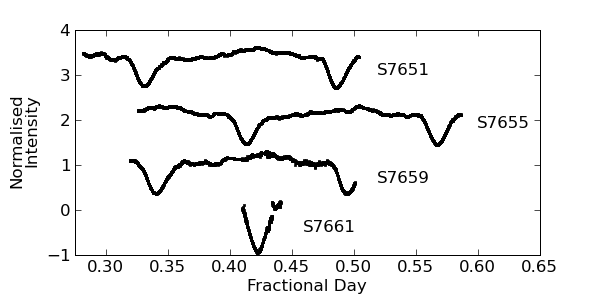
\includegraphics[bb=0 0 600 300,width=\columnwidth]{images/lightcurves.png}
 % lightcurves.png: 600x400 pixel, 72dpi, 21.17x14.11 cm, bb=0 0 600 400
\caption[Lightcurves of EC2117-54 for 16-19 August 2006.]{Lightcurves of EC2117-54 for 16-19 August 2006. They are in chronological order from top to bottom. They have been vertically displaced by arbitrary amounts for display purposes.}
\label{lightcurves}
\end{center}
\end{figure}

%#############################################################################################################################

\subsection{Ephemeris}

\label{ephemeris_section}

The August 2006 observations do not span a large enough period to precisely determine the orbital period from eclipse timing. Observations made some years earlier \citep{WWP} were retrieved from the archive and used to calculate the eclipse ephemeris. EC2117-54 shows partial eclipses, therefore only the accretion disk is being eclipsed. Because the accretion disk is subject to non-uniform variations of various causes, the eclipse profile is not the same for every eclipse. Measurement of the times of eclipse minima is therefore difficult because an identical function cannot be fitted to all eclipse profiles.

The eclipse minimum was located by finding the lowest point of a spline fitted to the eclipse. A spline fitting every 20 data points was used to find a smoothed version of the eclipse. This calculation was performed using a program written in the \texttt{Python} language.



% took the following approach,Fit a cubic spline through every $N$ datapoints in the eclipse.
% Evaluate the spline.
% Find the minimum value of the spline using a minimum slope algorithm.

%#############################################################################################################################

\begin{figure}
\begin{center}
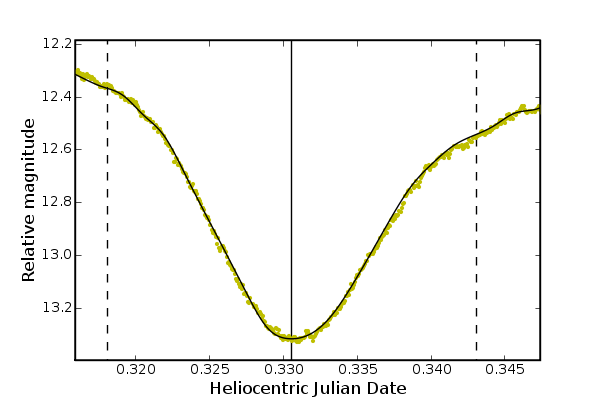
\includegraphics[width=0.85\columnwidth,bb=0 0 600 400]{images/eclipseminimum.png}
 % eclipseminimum.png: 600x400 pixel, 72dpi, 21.17x14.11 cm, bb=0 0 600 400
\caption[Measurement of eclipse minimum]{The plot shows the first eclipse in run S7651 (yellow/grey dots), the superimposed smoothing spline (solid black curve) and the date of the measured minimum (solid black vertical line). The broken lines on either side of the solid black vertical line are the limits between which the software finds the minimum. The magnitudes are instrumental. The number 2453964 has been subtracted from the Heliocentric Julian date.  }
\label{eclipseminimum}
\end{center}
\end{figure}

%#############################################################################################################################

Figure \ref{eclipseminimum} shows an example of the smoothing spline fitted to an eclipse and the corresponding minimum value found using this method. This is then repeated for all of the eclipses. Careful records must be kept of the number of eclipses that occurred after the first eclipse, to ensure that no cycle slips occur. Cycle slips show up as big residuals in the least-squares calculation. 

A first order function is then fitted to the eclipse times using least-squares to derive a precise value of the period. A parametric least-squares adjustment was used to estimate the period and its standard error. The method is outlined below.

The function to be fitted is written in the following form: $$  v = Ax - l $$ where $x$ contains unknowns, $v$ contains the residuals, $l$ contains the measured values and $A$ contains the coefficients of the unknowns. It can then be shown that the best-fit values of $x$ are given by $$ x = (A^{T}A)^{-1}A^{T}l $$ where $A^{T}$ denotes the matrix transpose of $A$. 

It can also be shown that the error estimates can be calculate from the following relation, $$ \Sigma_{xx} = \sigma^{2}_{0} \Sigma $$ where $$ \Sigma = (A^{T}A)^{-1} $$ and $$ \sigma^{2}_{0} = \frac{v^{T}v}{n-u} $$ where $n-u$ is the degrees of freedom of the solution. The matrix $ \Sigma_{xx} $ is known as the \textit{variance-covariance} matrix. The diagonals in this matrix contain the variances of the unknowns and the off-diagonal terms contain the covariances.

%#############################################################################################################################

\begin{figure}
\begin{center}
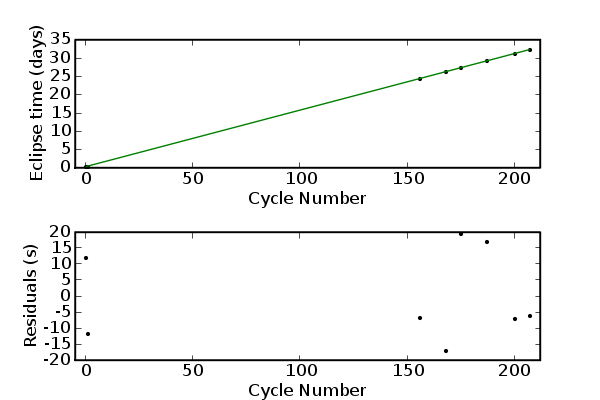
\includegraphics[width=0.80\columnwidth,bb=0 0 600 400]{images/ephemplot.png}
% ephemeris.png: 600x400 pixel, 72dpi, 21.17x14.11 cm, bb=0 0 600 400
\caption[Plot of Eclipse times versus cycle number of archival data]{The top plot shows eclipse times (in days) versus cycle number and the best-fit ephemeris, see Equation \ref{archive_ephem}. The bottom plot shows the residuals after the best-fit line has been subtracted.  The plots are based on the 2003 archival data.}
\label{ephemeris}
\end{center}
\end{figure}


\begin{figure}
\begin{center}
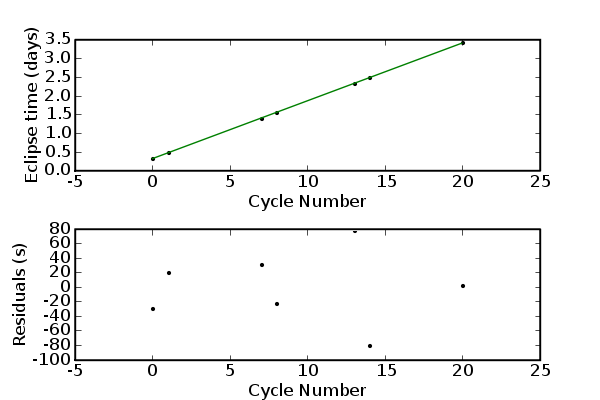
\includegraphics[width=0.80\columnwidth,bb=0 0 600 400]{images/ephem_plot_aug_data.png}
% ephemeris.png: 600x400 pixel, 72dpi, 21.17x14.11 cm, bb=0 0 600 400
\caption[Plot of Eclipse times versus cycle number of August 2006 data]{The top plot shows eclipse times (in days) versus cycle number and the best-fit ephemeris, see Equation \ref{aug_ephem}. The bottom plot shows the residuals after the best-fit line has been subtracted. The unit on the ordinate is seconds. The plots are based on the August 2006 data.}
\label{ephemeris_aug}
\end{center}
\end{figure}

%#############################################################################################################################

% The result from this method gives the period as $$ P = 13351.06 \hspace{4pt}s \pm 0.07 \hspace{4pt}s $$ where all the units are in seconds. See Figure \ref{ephemeris}.  

The ephemeris calculated from the archival data is given by
\begin{equation}
	\textrm{HJD}\:\: 2452525.374416 \pm 2 \times 10^{-4} + 0.154525E \pm  1\times 10^{-6}.
\label{archive_ephem}
\end{equation}

The bottom panel of Fig. \ref{ephemeris} shows the residuals of best fit ephemeris based on the 2003 archival data.  After this has been done for all the available eclipses, the resulting eclipse times and cycle numbers are plotted (see top panel of Fig. \ref{ephemeris}). Over the timescale of these measurements ($\approx$ 30 days), the eclipse times versus cycle number is a straight line.

The zero-point for the 2006 eclipse ephemeris was recalculated on the first eclipse of run S7651 and the new ephemeris is

\begin{equation}
	\textrm{HJD}\:\: 2453964.330709 \pm 4 \times 10^{-4} + 0.154525E \pm  1\times 10^{-6}.
\label{aug_ephem}
\end{equation}

The ephemerides are given in Heliocentric Julian Date. The orbital period and all errors are given in days. The errors are $1\sigma$ errors found from a least-squares fit. The orbital period and its error are those calculated from the 2003 archival data. Figure \ref{ephemeris_aug} displays the residuals of the ephemeris calculation based on the August 2006 observations. The residuals from the August 2006 fit contain 2 points with residuals that are much larger than the other eclipses. The ephemeris is measured using the minimum brightness during eclipse. The minimum brightness during eclipse in cataclysmic variables may occur at imprecise times due to flickering, noisy observations and other factors causing a non-uniform brightness distribution in the accretion disk.

The calculations were made using a program written using the \texttt{Python} programming language and the extension libraries, \texttt{Scipy} and \texttt{Matplotlib}. The spline minimum was calculated using the \texttt{Scipy} function, \texttt{fminbound}.

\section{Methods}
\subsection{Flattening of Lightcurves}

\label{flat_section}

The photometric observations were made in order to identify certain periodic phenomena in the brightness of the object. This was done using the standard method of Fourier analysis techniques. Periodograms of the lightcurves were calculated and the DNOs and lpDNOs were identified as peaks above the noise level. However, since the object undergoes an eclipse approximately every 3.708 hours, large low-frequency peaks appear in the periodograms that can suppress low amplitude peaks in the periodogram. This is illustrated in the periodogram shown in the bottom panel of Fig. \ref{unflat}. The lightcurves were flattened to remove variations in the brightness profile that are caused by the object's orbit.

All lightcurves were converted to intensity units and normalised their mean value. This allows for direct comparison of oscillation amplitudes between runs that is not dependent on the magnitude zero-point.

Different methods to remove the long period (orbital) variations from the lightcurves were investigated. The first method involved fitting a smoothing spline to the lightcurve and then subtracting it. This method removed the slow variations quite well but involved manual fitting of the spline to each lightcurve. In addition, this method gives no guarantee that periodic phenomena are not altered by the subtraction of the smoothing spline. This method was therefore deemed unsatisfactory.

Fast Fourier Transforms (FFTs) were used to remove the long period variations from the lightcurves. This requires the lightcurves to be sampled at regular intervals, which is not necessarily the case in astronomical observations. The lightcurves that contain gaps were interpolated to a regular grid using linear splines. The FFTs of the lightcurves were calculated. The positive and negative frequency terms corresponding to the long period signals were then set to zero, after which the inverse Fast Fourier Transform was calculated. This returns the lightcurve with the orbital variation and other longer period signals removed. Signals with a period longer than 30 minutes were removed because the rapid oscillations of interest have periods much shorter than this. This method resulted in flattened lightcurves with significant edge effects, caused by the discontinuity at the endpoints of the lightcurve i.e. the values of the lightcurve did not tend to zero at the start and end. For this reason, this method was also deemed unsatisfactory.

The method that was ultimately decided on involved the use of digital infinite impulse response (IIR) filters. This is the optimal way of removing unwanted frequencies from a signal. It has the advantage that the filter response, i.e. the attenuation as a function of frequency, is known. A ``Chebychev'' filter of Type I was used to construct a high-pass filter with a passband from 144 cycles/day, a transition-band between 100 and 144 cycles/day and a stopband below 100 cycles/day. The minimum attenuation in the stop band is 15 dB and the maximum attenuation in the pass band is 0.1 dB. A \texttt{Python} program using the \texttt{Scipy} package was used to implement this filter.

Figure \ref{unflat} shows a raw lightcurve and its periodogram. The noise level is at $\sim 0.1\%$ and no significant peaks at higher frequencies can be discerned. Figure \ref{flat} shows the same lightcurve from before, after it has been flattened with the IIR filter and its periodogram. The noise level is much lower than before ($< 0.001$) and the shorter period peaks can now clearly be identified.



%######################################################################################################################
\begin{figure}
\begin{center}
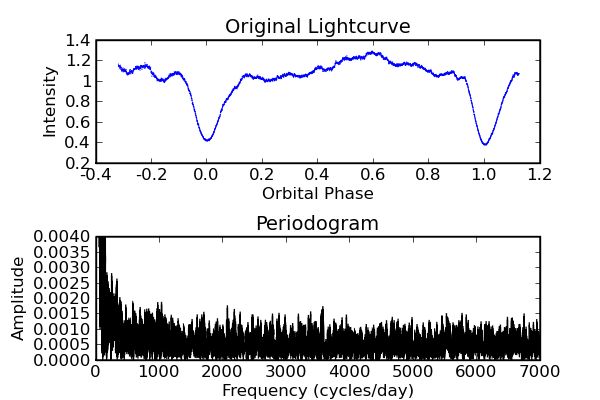
\includegraphics[width=0.80\columnwidth,bb=0 0 600 400]{images/unflattened.png}
 % unflattened.png: 600x400 pixel, 72dpi, 21.17x14.11 cm, bb=0 0 600 400
\caption[Original lightcurve and periodogram]{The original lightcurve of run S7651 and its periodogram. The periodogram is totally dominated by low-frequency noise and no details can be discerned.}
\label{unflat}
\end{center}
\end{figure}

%######################################################################################################################
%######################################################################################################################

\begin{figure}
\begin{center}
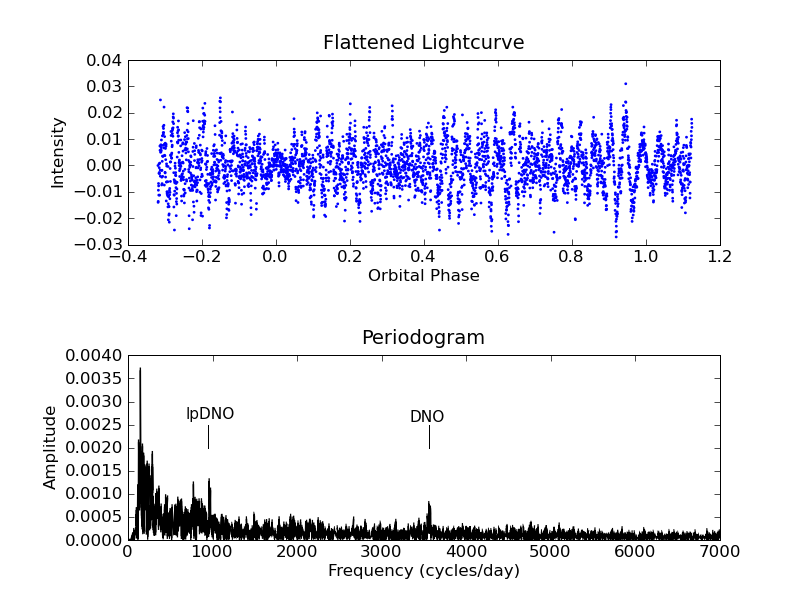
\includegraphics[width=0.80\columnwidth,bb=0 0 600 400]{images/flattened.png}
% flattened.png: 600x400 pixel, 72dpi, 21.17x14.11 cm, bb=0 0 600 400

\caption[Flattened lightcurve and periodogram]{The ``flattened'' lightcurve of run S7651 and its associated periodogram. Details in the periodogram can now be identified. Note the DNO peak at $\approx 3600$ cycles/day and lpDNO peak at $\approx1000$ cycles/day. The lightcurve was filtered using the IIR-filtering method described in Sect. \ref{flat_section}. }
\label{flat}
\end{center}
\end{figure}

%######################################################################################################################

% The lightcurves were ``flattened'' by calculating a smoothing spline fitting every $N$ points. The spline was then evaluated at the same times the observations were made at. The resulting points obtained from the spline were subtracted from the lightcurve to produce the ``flattened'' lightcurve. Cubic splines were again used for this operation. They were typically fitted to every 40 - 80 points (corresponding to 240 - 480 seconds). See Figure \ref{splineandflat} for an example.


\subsection{$O-C$ Diagrams}

\label{ominc_section}

In order to study the evolution of DNOs and lpDNOs, it is necessary to track the changes in their amplitude and phase as a function of time. This was done for this project using the following technique.

The lightcurves were flattened using the digital filtering technique described in Section \ref{flat_section}. The periodogram of the flattened lightcurve was then calculated and the frequencies at which the DNO and lpDNO peaks occurred were noted. An \textit{Observed - Calculated} ($O-C$) diagram was then plotted of the DNO or lpDNO at the frequencies found in the periodogram.

%#############################################################################################################################

\begin{figure}
 \centering
 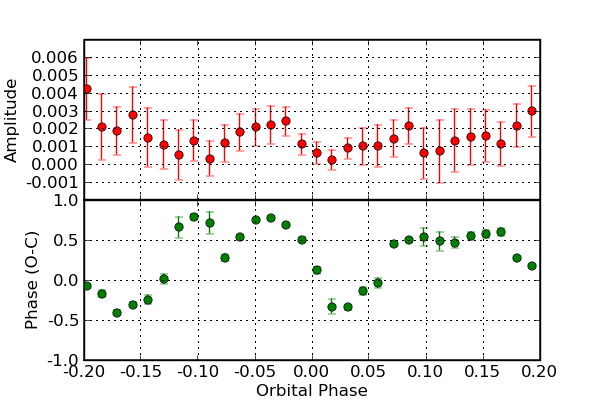
\includegraphics[width = 0.8\columnwidth, bb=0 0 600 400]{images/august_phot/S7651/S7651_24.30.png}
 % vel_ew.png: 1179666x1179666 pixel, 0dpi, infxinf cm, bb=0 0 600 400
 \caption[$O-C$ diagram around the first eclipse of run S7651.]{$O-C$ diagram around the first eclipse of run S7651. The phase was calculated relative to a signal with constant period of 24.30s (3555.56 cycles/day) using 15 cycles and 50\% overlap.  }
 \label{OC_example}
\end{figure}

%#############################################################################################################################

The $O-C$  diagrams are calculated by fitting a \textit{sine} function with the DNO period to overlapping segments of the lightcurve. The amplitude and the phase of the \textit{sine} function are allowed to vary. Their time-evolution can therefore be studied. The amount of overlap was chosen to be $50\%$, in order to minimise fitting error and to sample the lightcurve at closer intervals. Each segment typically contains $5$ to $40$ cycles of the variation under inspection. Knowing the sampling rate of the data, the frequency to be studied and the number of cycles to use in the process, it is trivial to calculate the number of data points to use for a segment. The fitting function used for the $O-C$ diagrams is $$y(t) = Acos(2\pi Ft) + Bsin(2\pi Ft)$$ where $F$ is frequency, $$Amplitude =\sqrt{A^{2} + B^{2}} $$ and $$ \phi = arctan(\frac{-B}{A}) $$
The amplitude and phase were then plotted as a function of time. Figure \ref{OC_example} shows the $O-C$ diagram for a DNO in run S7651. The fitting was done using the method described in section \ref{ephemeris_section}.

%#############################################################################################################################

\begin{figure}
 \centering
 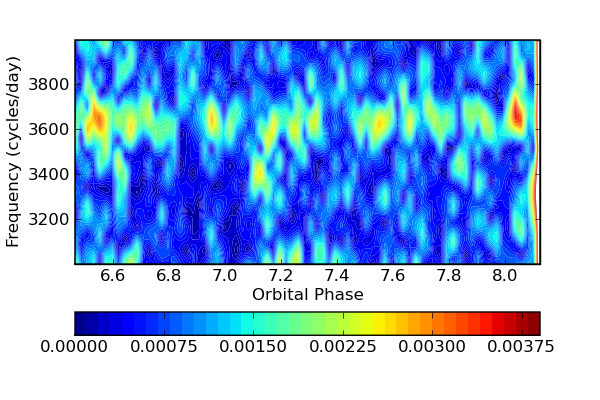
\includegraphics[width = 0.8\columnwidth, bb=0 0 600 400]{images/august_phot/S7655/S7655_DNO_trailed_FT.png}
 % vel_ew.png: 1179666x1179666 pixel, 0dpi, infxinf cm, bb=0 0 600 400
 \caption[Spectrogram for run S7655.]{A spectrogram for run S7655 around the $\sim3600$ cycle/day frequency. The color-bar shows the amplitude values in normalised intensity.  }


 \label{trailed_ft_example}
\end{figure}

%#############################################################################################################################


Examination of $O-C$ diagrams may reveal changes in the frequency and amplitude of an oscillation. A change of frequency will show up as a slope change on the $phase$ versus $time$ plot.

\subsection{Spectrograms}
\label{spectrogram_section}
A different way of looking at frequency and amplitude changes in a signal is to use a spectrogram. The spectrograms used in this analysis were computed by calculating periodograms of segments of a lightcurve with consecutive segments overlapping by 50\%. The periodograms were then plotted in an image with the vertical axis displaying frequency, the horizontal axis displaying time and the image value displaying amplitude. The time for each periodgram (i.e. column) was calculated by taking the average value of the times in the segment. See Fig. \ref{trailed_ft_example} for an example. Periodograms were calculated using the algorithm in \cite{kurtz_ft}.








%#############################################################################################################################

\begin{figure}[t]
\begin{narrow}{-0.75	in}{0in}
\begin{tabular}{lr}
 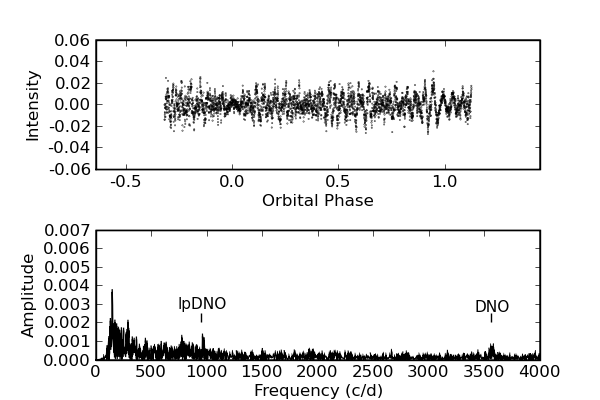
\includegraphics[width = 0.6\columnwidth, bb=0 0 600 400]{images/august_phot/S7651/S7651.png} & 
 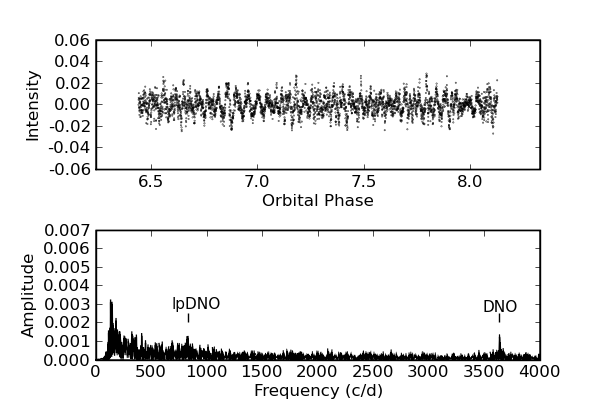
\includegraphics[width = 0.6\columnwidth, bb=0 0 600 400]{images/august_phot/S7655/S7655.png}  \\
 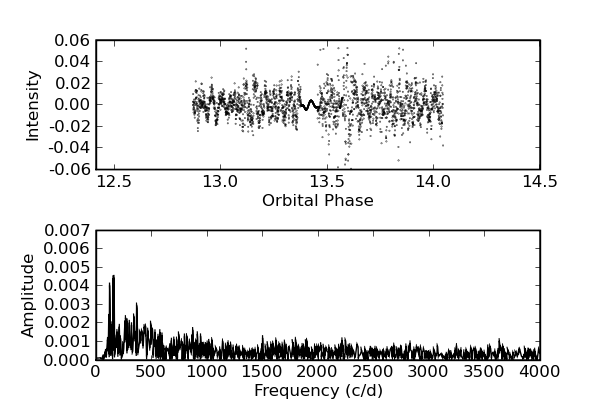
\includegraphics[width = 0.6\columnwidth, bb=0 0 600 400]{images/august_phot/S7659/S7659.png} &
 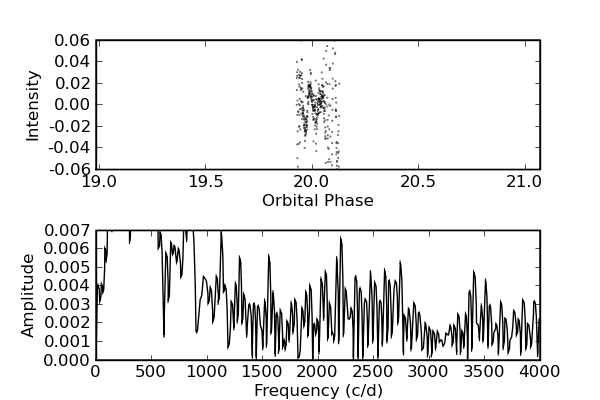
\includegraphics[width = 0.6\columnwidth, bb=0 0 600 400]{images/august_phot/S7661/S7661.png}
\end{tabular}
\end{narrow}
\caption[Flattened lightcurves and periodograms of EC2117-54.]{Flattened lightcurves and periodograms 
of EC2117-54. Clockwise from Top-left: Run S7651, S7655, S7661, S7659.} 
\label{ec2117_zcha}

\end{figure}

%#############################################################################################################################



\section{Analysis}

\subsection{Rapid Oscillations in August 2006 photometric lightcurves}
\label{ro_phot_lc}

Lightcurves from all 4 nights were flattened using the method described in section \ref{flat_section}. Periodograms were then calculated in order to identify any DNOs and lpDNOs. No search was made for QPOs because of their highly non-stationary nature. The filtering process may also introduce false signals into the lightcurve because the filter-cutoff is very close to the expected QPO period. Some of the flattened lightcurves contain sections that resembles QPOs (see top right panel of Fig. \ref{ec2117_zcha} for an example). For the above mentioned reasons these signals were ignored.  A more complete survey for them can be made using methods that incorporate non-stationarity of signal \citep{blackman}. The algorithm in \cite{kurtz_ft} was used to calculate the periodograms shown in Fig. \ref{ec2117_zcha}. The DNO ($\sim3600$ cycles/day) and lpDNO($\sim1000$ cycles/day) spikes in the periodogram can clearly be seen in run S7651 and S7655. On the third night (Run S7659) the DNOs and lpDNOs were not visible. Run S7661 was hampered by cloud and only a very short observing run was possible. The data from this run were not used in any further analyses. The DNOs and lpDNOs identified in the photometric lightcurves are shown in Table \ref{RO_table}.

%######################################################################################################################

\begin{table}
\begin{scriptsize}
\centering
\caption[Rapid Oscillations in photometry]{Rapid Oscillations in photometry.}
% use packages: array,supertabular
\begin{tabular}{rccccc}
\hline \hline\\
Run    & DNO period & DNO freq      & lpDNO period & lpDNO freq     \\ 
       & (s)        &  (cycles/day) &  (s)         &  (cycles/day)   \\ 
\\\hline \\
S7651$^{a}$  & 24.30, 24.12 [0.01] & 3555.56, 3582.09 [0.60] &  89.94 [0.01]  &  964.64 [0.60]  \\ 
*S7655$^{a}$ & 23.77 [0.30] & 3634.84 [0.01] & 104.2 [0.01] & 829.17 [0.30] \\ 
S7659$^{a}$  & --- & --- & --- &---\\ 
S7661$^{a}$  & --- & --- & --- &---\\
\hline\\
S6544$^{b}$  & 23.13 [0.03] & 3735.41 [0.70] & 95.68 [0.01] & 909.00 [0.40] \\
S6548$^{b}$  & ---   & ---     & ---    &---	\\
S6549$^{b}$  & 22.60 [0.10] & 3823.01 [2.20] & ---    &---	\\
S6551$^{b}$  & 22.66 [0.05] & 3812.89 [1.10] & ---    &---	 \\
S6555$^{b}$  & ---   & ---     & ---    &---	 \\
S6564$^{b}$  & 22.68 [0.16] & 3809.52 [3.60] & 95.39 [0.025] & 907.76 [2.40]  \\
S6570$^{b}$  & 22.63 [0.06] & 3817.94 [1.40] & 95.96 [0.014]  & 900.38 [1.30] \\
S6660$^{b}$  & 23.16 [0.15] & 3730.57 [3.40] & ---    &---     \\\\

\hline




\end{tabular}\\
* Observed in parallel with SALT high-speed spectroscopy. $^{a}$ August 2006 observing run. $^{b}$ Retrieved from archive. Errors are given in square brackets.

\label{RO_table}
\end{scriptsize}
% \caption{}
\end{table}

%######################################################################################################################



% DNO FTs

The periodogram of the flattened lightcurve of run S7651 (top left panel of Fig. \ref{ec2117_zcha}) shows evidence for a DNOs with periods at $\sim$24.3s and $\sim$24.1s. These oscillations are not present simultaneously. Calculating separate periodograms (not shown) for the first and second halves of the run reveals peaks at periods of $\sim24.3$s and $\sim24.1$s respectively.  (Table \ref{RO_table}). A very strong peak near 3640 cycles/day (23.7s) is seen in the periodogram (top right panel of Fig. \ref{ec2117_zcha}) of the flattened lightcurve of run S7655.






%######################################################################################################################

\begin{figure}[t]
\begin{narrow}{-1in}{0in}
% want 2x1 table with 2 Figs side by side on top and 1 on the bottom
\begin{tabular}{c}
    \begin{tabular}{cc}
    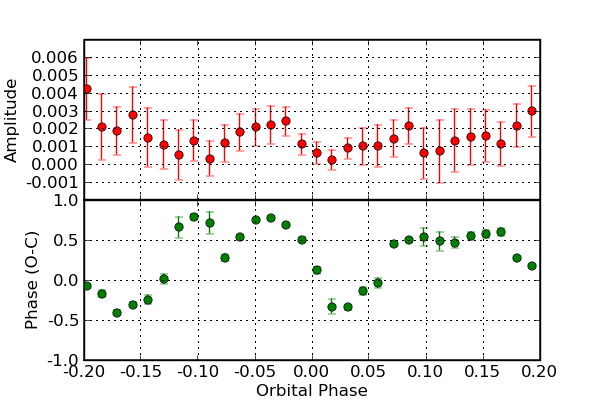
\includegraphics[width=0.65\columnwidth, bb=0 0 600 400]{images/august_phot/S7651/S7651_24.30.png} &
    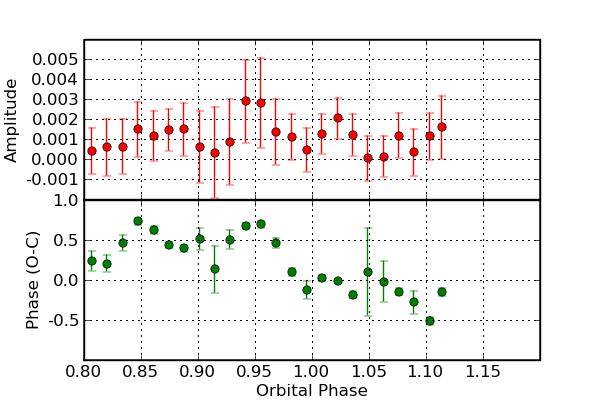
\includegraphics[width=0.65\columnwidth, bb=0 0 600 400]{images/august_phot/S7651/S7651_24.12.fixed.png}
    \end{tabular} \\
    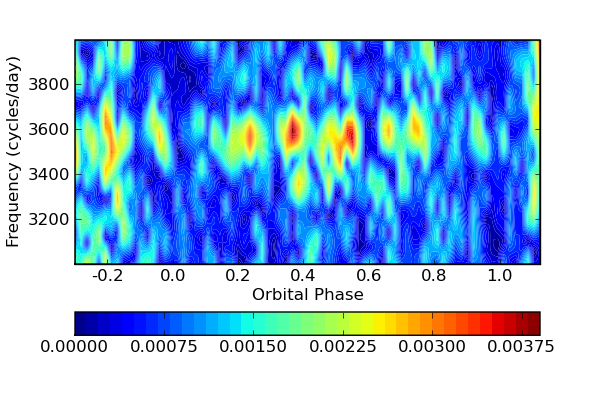
\includegraphics[width=0.65\columnwidth, bb=0 0 600 400]{images/august_phot/S7651/S7651_trailed_ft.png} 
%     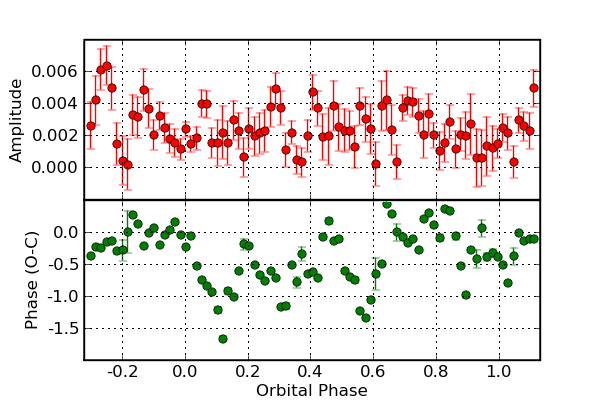
\includegraphics[width=0.42\columnwidth, bb=0 0 600 400]{images/august_phot/S7651/S7651_89.94.png}
\end{tabular}
\end{narrow}
\caption[$O-C$ Diagrams and spectrograms of DNO in run S7651]{$O-C$ Diagrams and spectrograms of DNOs in run S7651. The top left and top right panels show the $O-C$ diagrams around the first and second eclipses. They were calculated relative to signals with periods 24.3s and 24.12s respectively, using 20 cycles with 50\% overlap. The bottom panel shows the spectrogram centred on the DNO frequency for the entire run.}
\label{S7651_DNO}
\end{figure}

%######################################################################################################################




% lpDNO FTs

In the periodogram of the flattened lightcurve of run S7651 (top left panel of Fig. \ref{ec2117_zcha}, there is a very prominent peak near 960 cycles/day (89.95s). This is very close to $4\times\nu_{DNO}$ ($\nu_{DNO}= $ DNO frequency) and is therefore classified as a lpDNO. The periodogram of run S7655 showing a peak near 830 cycles/day (104.2s) can be seen in the top right panel of Fig. \ref{ec2117_zcha}. This is classified as a lpDNO and has the longest known period of all lpDNOs observed in this object. 

The DNOs and lpDNOs identified in the August 2006 runs occur at the expected periods, based on previous studies of this star \citep{WWP}. The DNOs and lpDNOs have periods of $\sim23$s and $\sim90$s respectively.



% DNO O-C
The $O-C$ diagrams of the DNO in run S7651 (top panels of Fig. \ref{S7651_DNO}) show evidence of a systematic phase change during the eclipses. The same phase variation is not seen in both eclipses of run S7651. During the first eclipse (top left panel of Fig. \ref{S7651_DNO}) the phase starts at $\sim0.7$ before eclipse, changes by $\sim1$ cycle and returns to $\sim0.5$ after eclipse. Immediately before the second eclipse the phase starts at $\sim0.5$, decreases to a value of about -0.4, and returns to $\sim-0.5$ after eclipse.

In run S7655 the DNOs exhibit similar behaviour through eclipse. The $O-C$ diagrams for the two eclipses are shown in the top panels of Fig. \ref{S7655_DNO}. The top left and top right panels show the $O-C$ diagrams for the DNO during the first and second eclipses respectively. The phase changes by $\sim$ 1 cycle during the first eclipse and does not revert to the value that was present before eclipse but instead seems to decrease. During the second eclipse in run S7655 (top right panel of Fig. \ref{S7655_DNO}) the phase changes from $\sim0.0$ to $\sim-0.9$ in mid-eclipse and returns to $\sim0.0$ after the eclipse.



% lpDNO O-C
The $O-C$ diagram (top left panel of Fig. \ref{aug_lpDNOs}) shows the lpDNO to have an irregular phase which is most likely due to the low amplitude and the associated difficulty of tracking the lpDNO. The amplitude is higher than average at orbital phases $\sim$0.3 and $\sim$1.1. The $O-C$ diagram of run S7655 (top right panel of Fig. \ref{aug_lpDNOs}) shows a constant phase throughout the run (including throught the first eclipse) that is interrupted immediately before the second eclipse. The amplitude panel as well as the spectrogram display a seemingly periodic strengthening of the signal every $\sim$0.2 to $\sim$0.3 orbital phases. These increases in amplitude seem to occur at the same orbital positions as in run S7651. The reason for this is unknown and may be purely coincidental. Neither of the runs contain an lpDNO that remained stable for long enough to be tracked through an eclipse.




% O-C diagrams





% landscpe plots for S7655
%#############################################################################################################################

% \begin{landscape}
\begin{figure}
\begin{narrow}{-1in}{0in}
\begin{tabular}{c}
    \begin{tabular}{cc}
        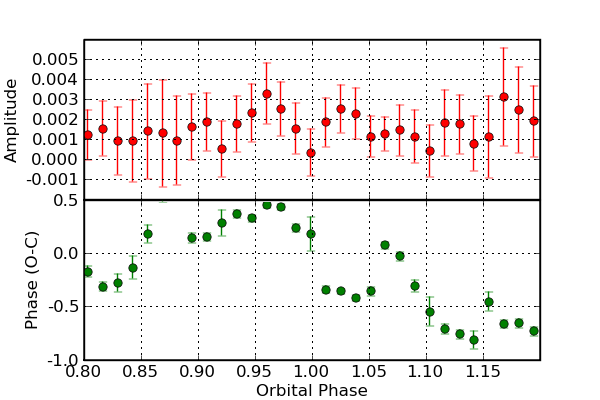
\includegraphics[width=0.65\columnwidth, bb=0 0 600 400]{images/august_phot/S7655/S7655_23.76_fixed_eclipse1.png} &
 	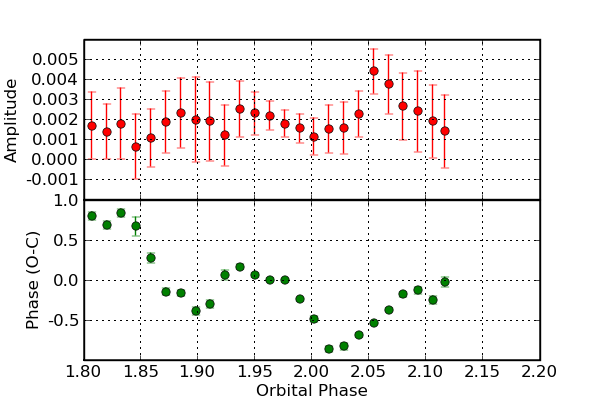
\includegraphics[width=0.65\columnwidth, bb=0 0 600 400]{images/august_phot/S7655/S7655_23.76_fixed_eclipse2.png}
    \end{tabular}  \\
 
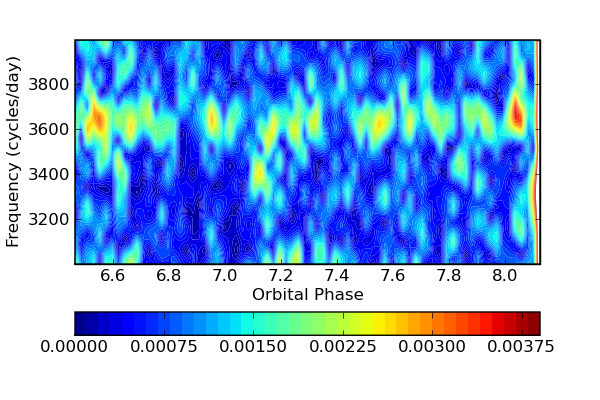
\includegraphics[width=0.65\columnwidth,bb=0 0 600 400]{images/august_phot/S7655/S7655_DNO_trailed_FT.png} 

\end{tabular}
\end{narrow}
% \end{displaymath}
\caption[$O-C$ Diagrams and Spectrograms for DNOs in run S7655]{$O-C$ Diagrams and Spectrograms for DNOs run S7655. The top left and -right panels show the $O-C$ diagrams the 23.76 s DNO during the first and second eclipse respectively. The bottom panel shows the spectrogram for the entire run centred on the DNO frequency for the entire run. The $O-C$ diagrams were calculated using 15 cycles with 50\% overlap. }
\label{S7655_DNO}
\end{figure}
% \end{landscape}

%#############################################################################################################################

\begin{figure}[t]
\begin{narrow}{-1in}{0in}
\begin{tabular}{cc}
 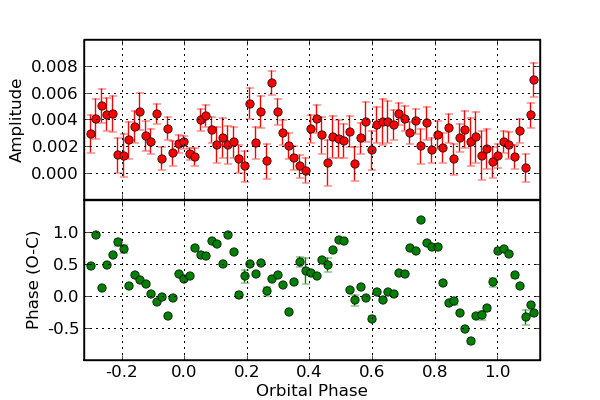
\includegraphics[width = 0.65\columnwidth, bb=0 0 600 400]{images/august_phot/S7651/S7651_89.95.png} & 
 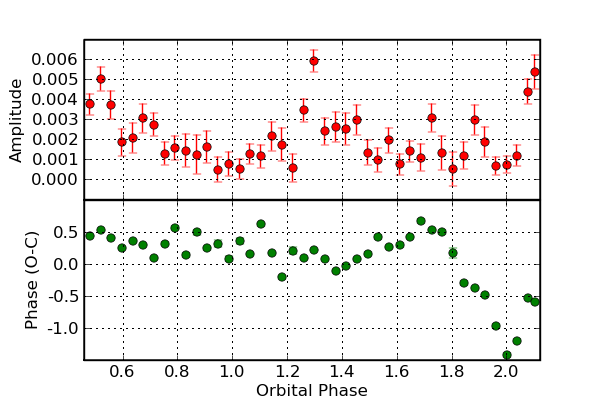
\includegraphics[width = 0.65\columnwidth, bb=0 0 600 400]{images/august_phot/S7655/S7655_104.2.png}  \\
 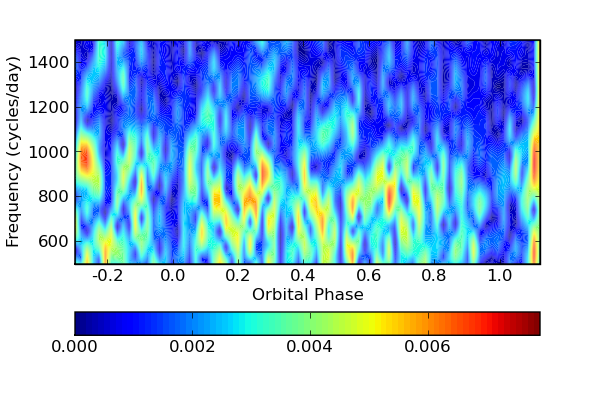
\includegraphics[width = 0.65\columnwidth, bb=0 0 600 400]{images/august_phot/S7651/S7651_trailed_FT_lpDNO.png} &
 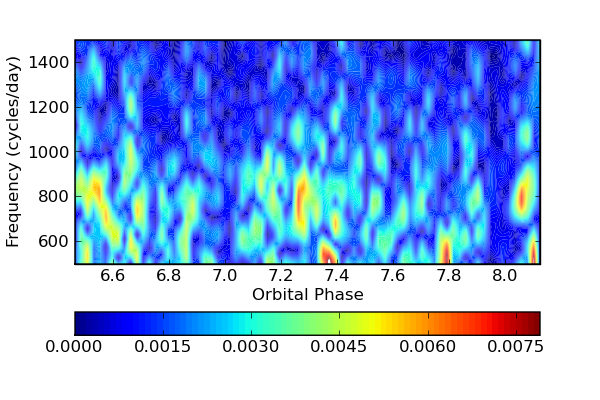
\includegraphics[width = 0.65\columnwidth, bb=0 0 600 400]{images/august_phot/S7655/S7655_lpDNO_trailed_FT.png}
\end{tabular}
\end{narrow}
\caption[$O-C$ diagrams and spectrograms of lpDNOs in EC2117-54]{$O-C$ diagrams and spectrograms of lpDNOs in EC2117-54. The left panels displays run S7651 and the right S7655.} 
\label{aug_lpDNOs}
\end{figure}




















% Z Cha



%#############################################################################################################################


Evidently the phase evolution of the DNO signal through eclipse is not visible at every eclipse. The fact that a systematic effect can be seen through eclipse suggests a geometrical origin and therefore the geometry of the system is not constant. The accretion disk, the accretion stream and the stream-disk impact zone are the only parts of the cataclysmic variable that can show changes on the timescale of an orbital cycle, and therefore one or both must have an integral part in this phenomenon. This is further discussed in Sect. \ref{photo_discussion}.



\subsection{Rapid Oscillations in archival photometric light-curves}
\label{ro_arc_phot_lc}

The discovery of systematic phase changes in the August 2006 lightcurves prompted a search for the same occurrence in data from the archive. Observations made during eclipse were retrieved and analysed using the same methods as the August 2006 data. Phase changes in the DNOs were identified in 4 of the 8 archival runs analysed (S6555, S6564, S6660 and S6570). The flattened lightcurves and their periodograms are shown in Fig. \ref{ec2117_archive}. Figures \ref{fig:ux_uma_OC} and \ref{fig:z_cha_OC} show average $O-C$ diagrams for every eclipse containing DNOs showing the two kinds of phase changes. Interestingly, the average $O-C$ diagram in Fig. \ref{fig:z_cha_OC} shows two phase changes. The first one, at orbital phase $\phi=0.9$, is shorter and more shallow than the second one ($\phi=1.05$) . This can also be seen in some of the $O-C$ diagrams of single runs. This is discussed in Sect. \ref{photo_discussion}.

A similar phase change was observed in the dwarf nova Z Cha during super-outburst by \cite{warner_brickhill}. A more modern lightcurve of Z Cha during outburst that contains DNOs was retrieved from the archive to look for the same phenomenon during eclipse. The lightcurve was flattened using the method outlined in Sect. \ref{flat_section}. Figure \ref{Z_Cha_OC} shows the filtered lightcurve and periodogram of run S6061 of Z Cha. Very strong DNOs can be seen in the periodogram (right panel of Fig. \ref{Z_Cha_OC}) at a frequency of $\sim$3500 cycles/day. This corresponds to a period of 25.15s. Examination of the $O-C$ diagram (left panel Fig. \ref{Z_Cha_OC}), calculated relative to a constant signal with a period of 25.15s, unfortunately does not show the phase changes, however, this is not surprising given the variable nature of the DNOs seen in EC2117-54.

%#############################################################################################################################

\begin{figure}
 \centering
 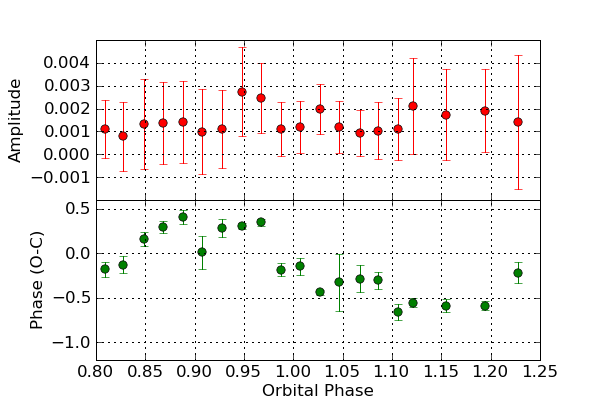
\includegraphics[width=0.7\columnwidth,bb=0 0 600 400]{images/averaged_OC/fixed_may2008/ux_uma_type/average_OC.png}
 % average_OC.png: 600x400 pixel, 100dpi, 15.24x10.16 cm, bb=0 0 600 400
 \caption[Averaged $O-C$ diagram of UX Uma-type phase change.]{Averaged $O-C$ diagram of UX Uma-type phase change. Diagram was calculated using data from run S6660, S7651 and S7655.}
 \label{fig:ux_uma_OC}
\end{figure}



\begin{figure}
 \centering
 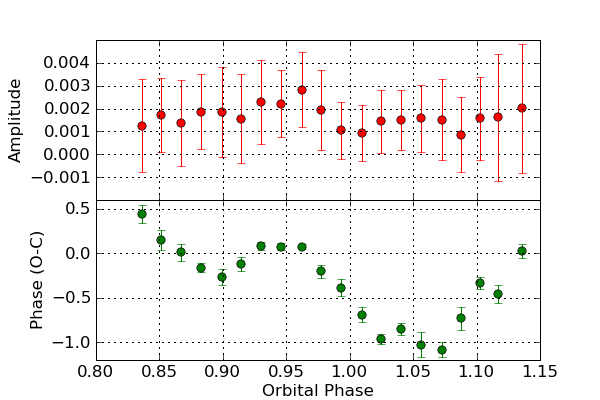
\includegraphics[width=0.7\columnwidth,bb=0 0 600 400]{images/averaged_OC/fixed_may2008/z_cha_type/average_OC.png}
 % average_OC.png: 600x400 pixel, 100dpi, 15.24x10.16 cm, bb=0 0 600 400
 \caption[Averaged $O-C$ diagram of Z Cha-type phase change.]{Averaged $O-C$ diagram of Z Cha-type phase change. Diagram was calculated using data from run S6555, S6564, S6570, S7651 and S7655.}
 \label{fig:z_cha_OC}
\end{figure}


\begin{figure}
 \centering
 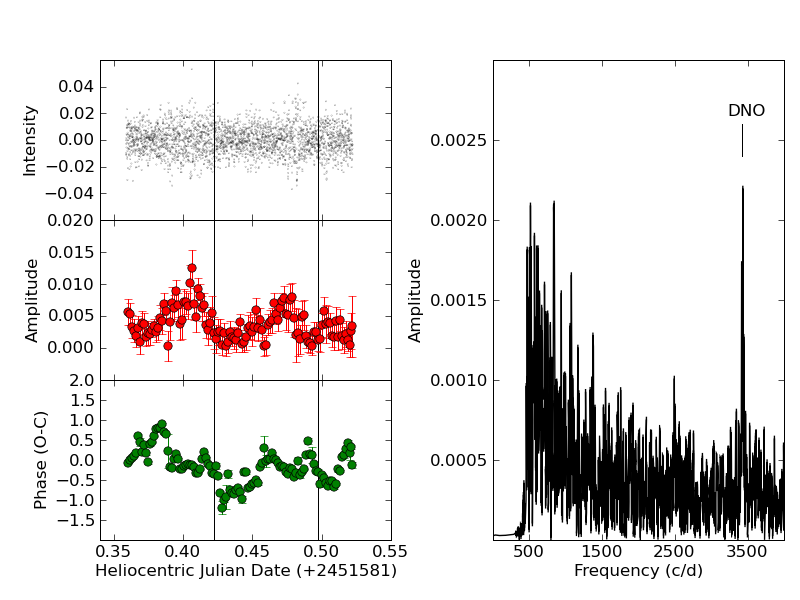
\includegraphics[width=\columnwidth,bb=0 0 800 600]{z_cha/z_cha_OC_FT.png}
 % z_cha_OC_25.13.png: 900x600 pixel, 100dpi, 22.86x15.24 cm, bb=0 0 600 400
 
 \caption[Filtered lightcurve,$O-C$ diagram and periodogram of Z Cha.]{Left: Top panel shows filtered lightcurve of run S6061 of Z Cha, middle and bottom panels contains amplitude and phase variations of the 25.15s DNO respectively. The solid vertical lines indicate times of mid-eclipse. The DNO phase change is not seen in this run. Right: Periodogram of filtered lightcurve with DNO peak marked. }
\label{Z_Cha_OC}
\end{figure}


\begin{figure}
\begin{narrow}{-0.25in}{1.5in}
\begin{tabular}{lr}
 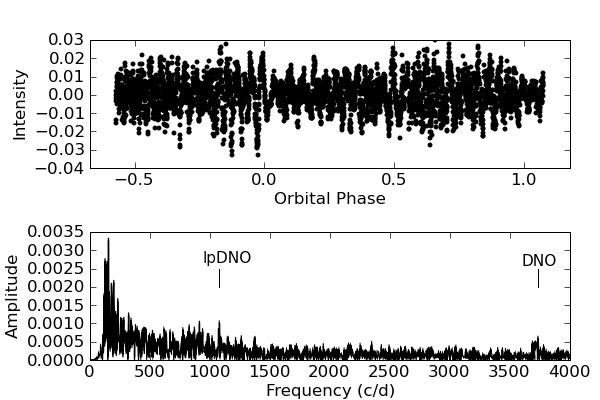
\includegraphics[width = 0.50\columnwidth, bb=0 0 600 400]{images/archive_phot/norm_int_eclipsing/S6544_c_FF.png} & 
 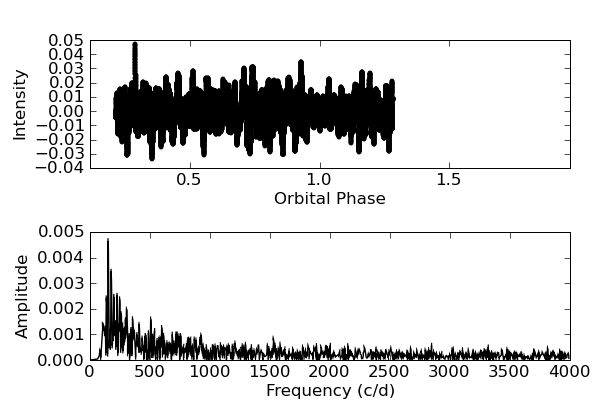
\includegraphics[width = 0.50\columnwidth, bb=0 0 600 400]{images/archive_phot/norm_int_eclipsing/S6548d_cc_FF.png}  \\
 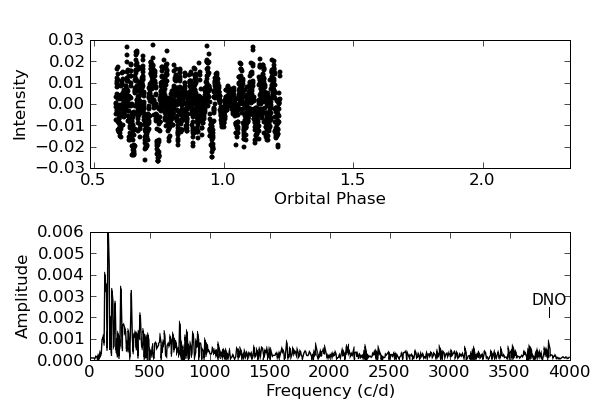
\includegraphics[width = 0.50\columnwidth, bb=0 0 600 400]{images/archive_phot/norm_int_eclipsing/S6549d_FF.png} &
 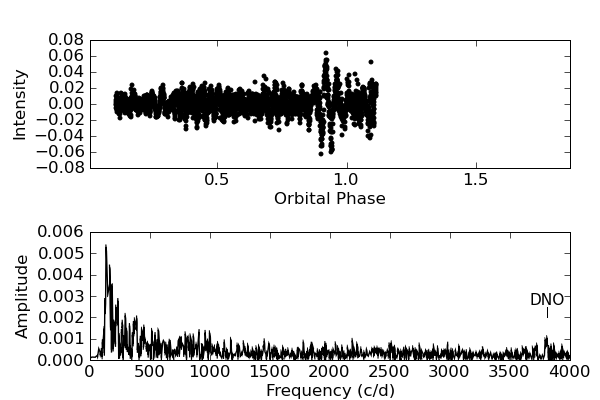
\includegraphics[width = 0.50\columnwidth, bb=0 0 600 400]{images/archive_phot/norm_int_eclipsing/S6551d_FF.png} \\
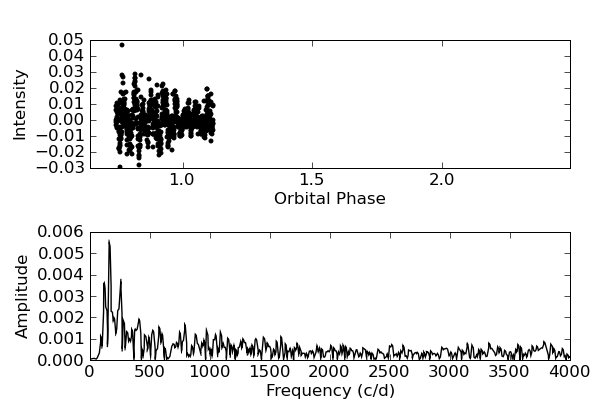
\includegraphics[width = 0.50\columnwidth, bb=0 0 600 400]{images/archive_phot/norm_int_eclipsing/S6555d_FF.png} &
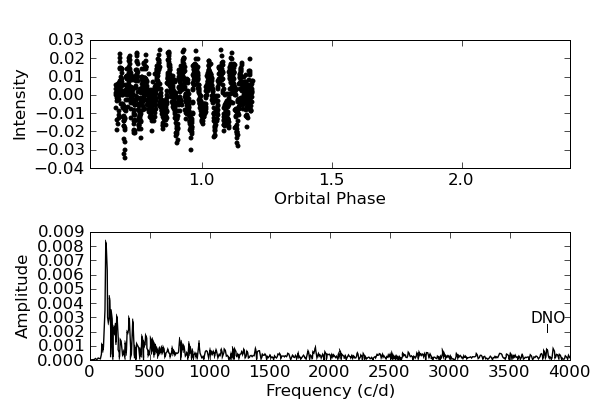
\includegraphics[width = 0.50\columnwidth, bb=0 0 600 400]{images/archive_phot/norm_int_eclipsing/S6564d_FF.png} \\
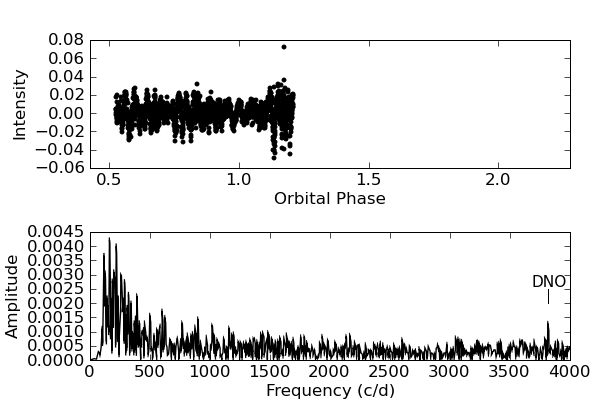
\includegraphics[width = 0.50\columnwidth, bb=0 0 600 400]{images/archive_phot/norm_int_eclipsing/S6570d_FF.png} &
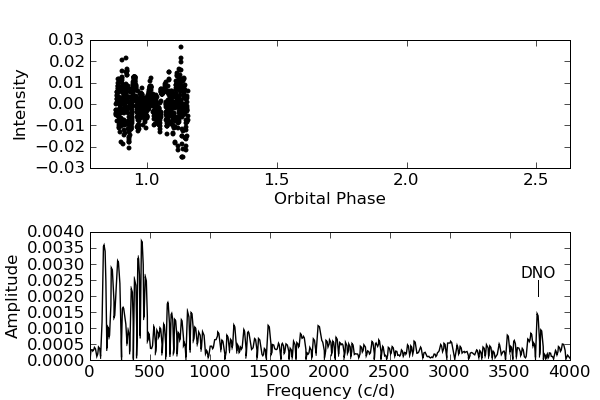
\includegraphics[width = 0.50\columnwidth, bb=0 0 600 400]{images/archive_phot/norm_int_eclipsing/S6660d_FF.png}

\end{tabular}
\end{narrow}
\caption[Flattened lightcurves and periodograms of EC2117-54.]{Flattened lightcurves and periodograms 
of EC2117-54. Clockwise from Top-left: Run S6544, S6548, S6551, S6564, S6660, S6570, S6555 and S6549.} 
\label{ec2117_archive}
\end{figure}


\begin{figure}
\begin{narrow}{-1in}{0in}


\begin{tabular}{cc}
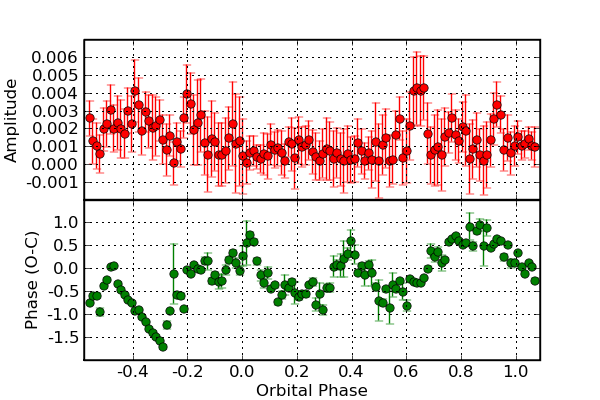
\includegraphics[width = 0.65\columnwidth, bb=0 0 600 400]{images/archive_phot/norm_int_eclipsing/S6544_23.13.png} &
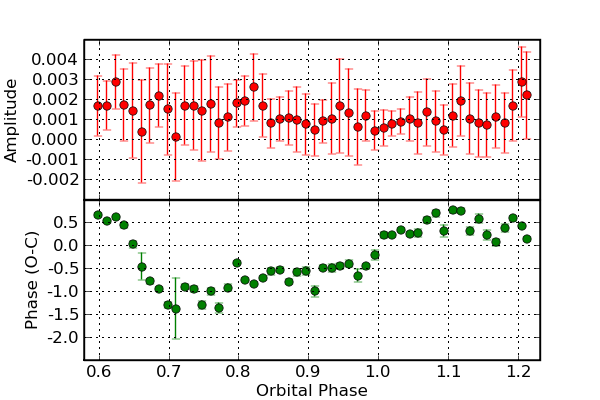
\includegraphics[width = 0.65\columnwidth, bb=0 0 600 400]{images/archive_phot/norm_int_eclipsing/S6549_22.60.png} \\
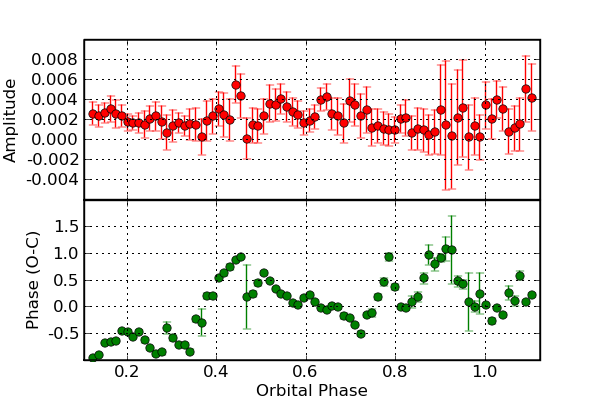
\includegraphics[width = 0.65\columnwidth, bb=0 0 600 400]{images/archive_phot/norm_int_eclipsing/S6551d_22.66.png} &
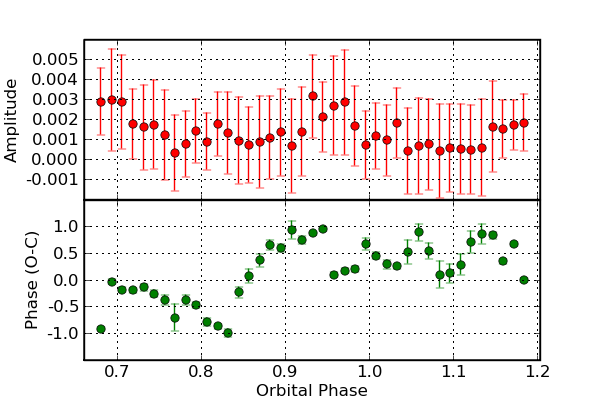
\includegraphics[width = 0.65\columnwidth, bb=0 0 600 400]{images/archive_phot/norm_int_eclipsing/S6564d_22.68.png} \\
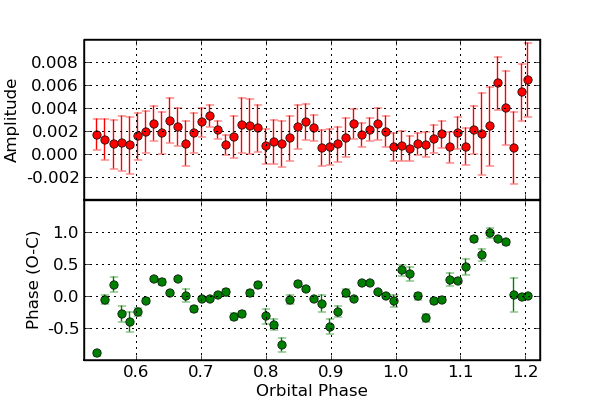
\includegraphics[width = 0.65\columnwidth, bb=0 0 600 400]{images/archive_phot/norm_int_eclipsing/S6570_22.63.png} &
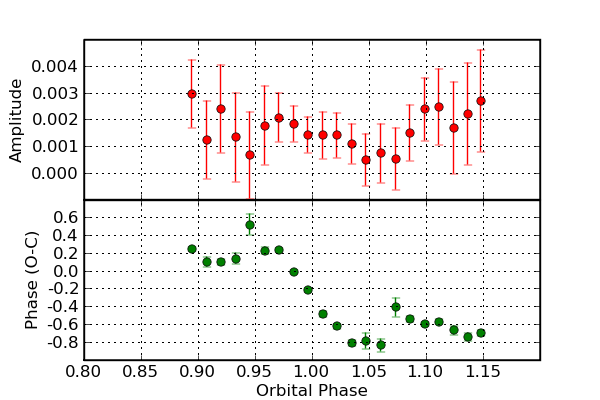
\includegraphics[width = 0.65\columnwidth, bb=0 0 600 400]{images/archive_phot/norm_int_eclipsing/S6660d_FF_OC.png} 
\end{tabular}
\end{narrow}
\caption[$O-C$ diagrams of DNOs in archive data.]{$O-C$ diagrams of DNOs in archive data. Clockwise from top left: Run S6544, S6549, S6564, S6551, S6660, S6570. All diagrams were calculated using 15 cycles with 50\% overlap. Phase panels were calculated relative to constant signals with periods as listed in Tab. \ref{RO_table}.} 
\label{ec2117_archive_OC}


\end{figure}





